\subsection{Editors}\label{sec:editors}

This section will describe the most relevant \acrfullpl{IDE} for \acrlong{emf} and the \gls{cloud}.

\subsubsection{Visual Studio Code}\label{sec:vscode}

\paragraph*{What it is}
Visual Studio Code (\gls{VSCode}) is a text editor and \acrfull{IDE} created by
Microsoft. The VSCode editor is based on the \gls{open source} software (OSS) called \emph{VS Code Project}.~\cite{helmingEclipseTheiaIDE2019} 
The VSCode editor has Microsoft-specific customizations, which makes it slightly different from the OSS project.~\cite{microsoftMicrosoftVscode2020} (This is analogous to the relationship between the \gls{open source} Chromium and the proprietary Google Chrome.)

\begin{figure}[htbp]  % order of priority: h here, t top, b bottom, p page
  \centering
  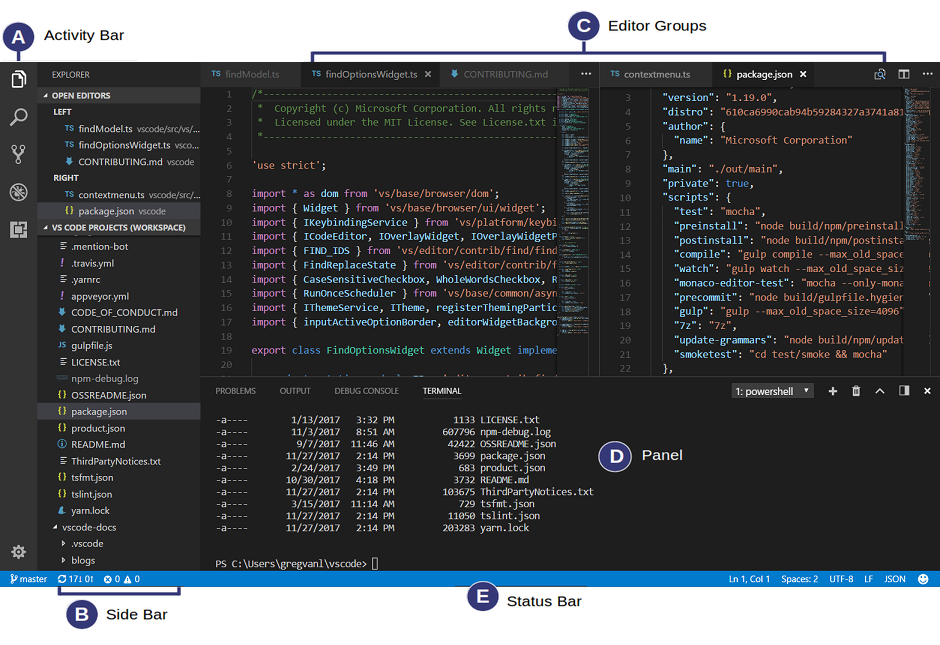
\includegraphics[width=\textwidth]{figures/vscode-ui}
  \caption[Visual Studio Code User Interface]{The user interface of Visual Studio Code.\cite{microsoftVisualStudioCode2020}}\label{fig:vscode-ui}
\end{figure}

\paragraph*{Intended use} Primarily an editor for textual programming languages.
VSCode has no support for diagrams or binary file viewers (like 3D models) out of the box. By default, it supports \texttt{Javascript}, \texttt{Typescript} and \texttt{Markdown}; common technologies related to web development.
VSCode can be extended to support other languages and editors, see \cref{chap:vscode-extension}.

VSCode runs as a desktop application, and uses Electron and javascript for its runtime.
The actual text editor in \gls{VSCode} is called \emph{Monaco}, and is separated out as a standalone package.

% What does it do?
% Who made it?
% Architecture

\subsubsection{Theia}\label{sec:theia}

\paragraph*{What it is}
\Gls{Theia} was created to be a framework for creating custom and
white-labeled \acrshortpl{IDE} and tools. Theia itself was not an IDE.~\cite{helmingEclipseTheiaIDE2019}
The project was originally started by TypeFox, but donated to the Eclipse Foundation.
It is free and fully \gls{open source}.
\Gls{Theia} is based on the same components as \gls{VSCode}, and uses Monaco as well.
The main uses of Theia now is as an editor for workspace software like \gls{Che} and \gls{Gitpod}.

% What does it do?
% Who made it?
% Architecture

\subsubsection{Eclipse IDE}
%TODO: write
% What does it do?
% Who made it?
% Architecture
